%\addcontentsline{toc}{chapter}{Development Process}
\chapter{Design}
On completion of my analysis and background planning for the project, I can now look at more detailed design for the application overview, and the individual component it comprises of. Becuase my application will present both a front-end GUI and back-end Javascript and WebGl, I will split my design into two sections. The reasoning for this is becuase I would prefer to have the GUI and logic of the application to be decoupled, so that the code can be changed in the Javascript easily without having to affect the user interface. Other than planning the application itself, it is also important I plan what key assisting services I use, such as how I intend on versioning my code, to how I will deploy my code.

\section{Overall Architecture}
As a summary of the architecture of my planned application, the best way to design in more detail is to lay out a primary design pattern. For the purpose of an application which will allow for user interaction, which will be processed by code in the back-end, I have decided to go ahead with a Model-view-controller approach. Using the MVC pattern means I can separate the GUI from the logic code as I wanted to, and have the GUI exists without knowledge of the back-end. This is also the same with the model, where the primary code for calculating manoeuvre movements and animations should be possible without knowledge of the view, but instead use the controller as a intermediary. See figure ~\ref{fig:mvc} for the MVC pattern I plan to use. 

\begin{figure}[h!]
  \centering
      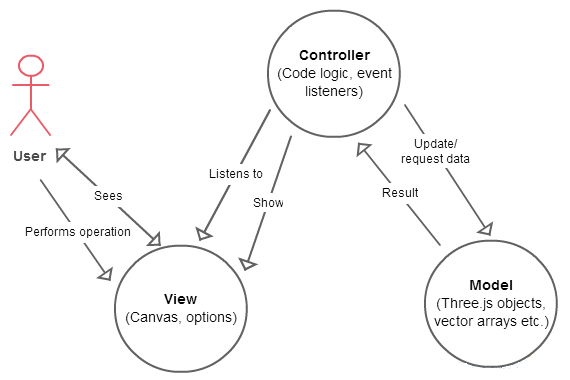
\includegraphics[width=0.8\textwidth]{images/mvc.png}
  \caption{Model View Controller diagram for my proposed application. Shows the planned interactions between different subjects within my application.}
  \label{fig:mvc}
\end{figure}

Because I have already chosen three.js as library of choice for creating any graphics and physics objects, these will already form my model or models. Each manoeuvre for instance will be reflected as a set of vectors which will form the shapes of the Aresti flight paths, and should be accessible and changeable through the controller to the view(in this case the canvas in my GUI).

The controller will be the most crucial part I implement, as it will need to be able to communicate with the three.js objects, the canvas disaplaying the animation, and detect controls from the user. For this piece of the pattern, I will enforce some other design patterns to 

Finally, the view will be represented as the canvas and controls on the web page. Since on both the canvas and the options menu can have an affect on the model, the controller will listen for changes on either, and then call the relevent operations to affect the model, and again reflect this back onto the view. The view will not know anything of the controller nor the model, so adding any new options or displayable information will be easier and not conflict with any current elements.

\section{Back-end logic and design}
The first of the two design categories concentrates on the JavaScript that will act as the functions to run each of the proposed features of the application. The code on this side will be responsible for maintaining contact with the GUI, and more importantly the WebGL canvas on the web page. To make the code be as maintainable and run effectively as possible, I will look into a variety of design patterns.

\subsection{Design patterns}
Because I am using a hybrid of waterfall and FDD at this stage of the project, using a changing range of design patterns for my JavaScript and GUI architecture is possible. Through the implimentation stage of this report, some of these may patterns mentioned may not be used anymore and replaced for different ones depending on changing requirements and progress. Using the implement, refactor and test iteration approach should allow for this.

The first design pattern that would be good useful relating to the controller is known as an observer pattern. The observer pattern means to listen on an event or events in an application, and then call the relevent action. The JQuery library, which I plan to use throughout any GUI related tasks will be of a great use here. This library will allow me to add simple listeners on elements on the web page, and set methods to be called on any click, hover or other events. In terms of how I will place this pattern in my archetecture, a standalone file will be responsible for listening to any options or menu changes, whilst another JavaScript file will be repsonsible for listening to the canvas events such as rotation or zoom.

The next design pattern I plan on implementing into my application relates again to the MVC archetecture I will be using. The builder pattern will allow me to append and edit any HTML on the page(such as options, checkboxes, loading content back into the OLAN input box) easily with data retreieved from the model. JQuery again should help to provide a means of changing content, becuase of more built-in method it comes with. There should be a handler class in my application specifically for controlling the page content.

A third design pattern which will be important when it comes to loading up the application will ensure that all the data nessecary to run the application is ready before the user can perform any actions. Known as the Lazy initialisation pattern, this is a style of coding that means whenever files or data is being loaded, the rest of the application should either wait, or prevent other relying features from being initialised. One motivation for the need for this pattern in my program is becuase of the vast amount of manoeuvre data, and model data for terrain or for aircrafts means that functionality such as animating and drawing flight paths on the canvas may be already ready for use from the user before all the data is ready. In this case, it could cause errors and even crash the application. Therefore, making sure that the application does not progress loading before data is ready is of great importance.

Although the previous design patterns have been chosen, others were considered when planning the application but were not suitible or better options were availible. One such pattern, the Mixin pattern allows JavaScript functions to be inherited from other classes or inner functions. For instance, these would be useful as a means of decreasing repition of functions. In my proposed application, I thoguht about the possibility of using a Mixin style architecture to allow functions that would draw both the manouevres on the canvas, and the manoeuvres on the movie-reel. The reason I have decided not to use this pattern falls to the issue that by making an object extend and hold code from elsewhere could make it harder to maintain, see where the function comes from, and uncertainty of location of any bugs I may come across while developing.

\subsection{Module diagram}
\label{sec:module}
Because much of the code I will be implementing will hold various Three.Js objects, I have decided that modulating methods and objects will be better than simulating classes seeing as JavaScript is a class-less language. This is a pattern known as the module pattern. Although this may appear less object orientated, modules allow for more robust archetecture where units of code can be separated and organised. Modules are slightly similar to classes in the way they can hide code that should not be accessable to other modules by encapsulates privacy. When code is modulated, and then that module is called upon by another, only a public API is returned, and other methods in that module are kept private from being used in other parts of the application. These private methods are good for use as supporting methods, holding such things as calculations, or private variables for getters and setters. Again, this is a similar case to the traditional class diagram.

There are currently a selection of libraries that allow for modules in JavaScript. The most promininent, and the one I would like to use is called RequireJS, which promises the increase in speed and quality of code. RequireJS works by dynamically loading JavaScript files on the fly, where the code has from the other module is usable once loaded into the module calling it. Once modules are loaded into an object form in whatever the developer needs to name it, its public variables and methods can then be accessed. See figure ~\ref{fig:module} on how modules are used. In my case, modules would be useful in enforcing the MVC pattern in the way that it will help towards hiding code between the view and the model. 

\lstset{language=JavaScript}
\medskip
\begin{lstlisting}[caption=Example showing how RequireJS loads in another module or Javascript file which in this case is loading up the util javascript module and naming it as object 'util' for use in the code]
require(["helper/util"], function(util) { 
	
	// This function can not be called by another module
	function private_function(){
		util.Method() // Can call public methods in the util file
	}
	return {
		public_function: function(){
			// can be called if this module is loaded into another
		}
	}
});
\end{lstlisting}
\label{fig:module}

In order to create a basis for modulating code, I should first look to seperate the features I listed in the analysis section of this report into categories. These categories will then help me to determine how I could structure my application in as best object orientated way as possible.

The categories I have been able to come to are:
\begin{itemize}
  \item Main- initiating other modules, beginning the application.
  \item Animation- Playing, and controlling speed, physics of animation.
  \item Loading manoeuvres at start of application.
  \item Saving and loading animations
  \item Cameras- Creating and controlling cameras movements
  \item GUI controlling- control and edit GUI controls, and appearence from back-end. Also including the possible movie reel live animatiion.
  \item Canvas controls- Allowing the user to move along the canvas, and zoom.
\end{itemize}

Now I have a stable list of categoried features, I am able to create a diagram shown in figure ~\ref{fig:mod} to represent what modulated layout my applicatioon will use. Becuase of the way modules handle public and private variables, have public and have private methods, means that this is very reminiscent of a standard class diagram.

\begin{figure}[h!]
  \centering
      %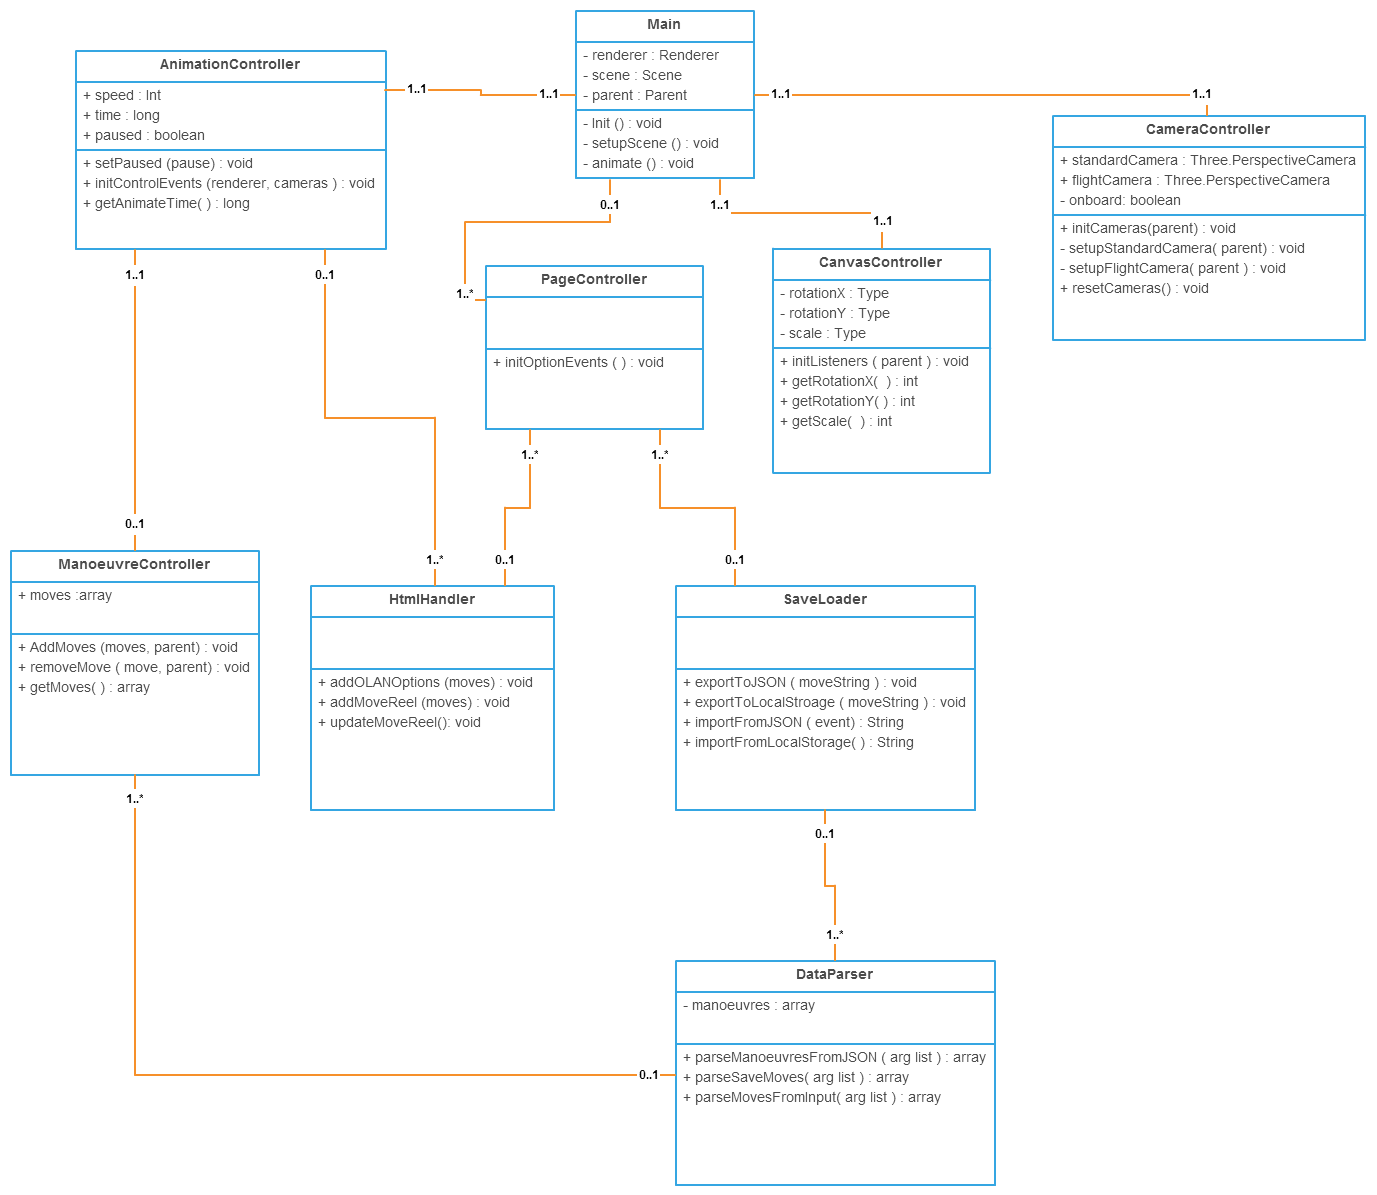
\includegraphics[width=0.8\textwidth]{images/mod.png}
  \caption{Module diagram displaying the various communications between modules, and how they are connected to the GUI in the MVC way.}
  \label{fig:mod}
\end{figure}

This module diagram shows what will be the communications between modules in the application, providing insight into what each module should contain in terms of important variables and methods. Ensuring that only modules that require certain peices of information from another module has sole access is important to reinforce the module pattern mentioned earlier. It should be noted here that although the diagram shows the main modules that will oversee most of the features of the application, when implementation occurs later on in the project, more modules or JavaScript files may be added to support or lighten the load of functions. This is supported by the good practice of \textbf{keeping files and functions short and concise} for easier maintenence and readability. The following descriptions have been kept brief, and key connections within the diagram discussed.

The first module propsed from the diagram will be the module entitled 'Main', which will be responsible for setting up the application, and hold onto key variables such as the renderer and scene objects to allow for anything to be drawn and animated on the canvas. This module will be called from the HTML and then will begin any nessecary calls to set up the listeners for the cameras, canvas and options. The most importat call will be the call to set up the animation controller module. 

Following on, the animation controller module will be one of the largest and most important parts of the overall architecture, as it will be responsible for both animating flight paths, loading up the OLAN manoeuvres at start of the application, and relating any actions from the user to do with OLAN selections or playing and pausing, as well as chaning animatiton speeds. 

The animation controller module will be in communication with the manoeuvre controller, which will be a logic heavy class because of the calculations it will require to compute and construct the sets of vectors of the Aresti shapes representing each OLAN notation. As the diagram shows, the application will first get the user OLAN input from the webpage via the HTML handler module, then search via the dataParse module and create the manoeuvres array object within the manoeuvre controller holding all the calculated manoeuvres, and return this in a 'get' method to the animation module for placing on the canvas.

As mentioned earlier, the HTML handler module will be the first means of contact to the user of the application, retreving input from the OLAN box, getting values of any checkboxes, and also setting any values. This module will be using the JQuery library as well as the Handlbars library as the primary way to communicate with the front-end, by diectly referencing ID's of divs on the webpage.

Two other controllers that should be mentioned are the camera dna canvas modules. Both modules will be resposible for setting up their elements when the applicaton starts up (including the different sets of cameras, locations, lighting and ground effects) and for listening to evens on both of their respective related front-end sections. Whilst the canvas module will only need to listen for events on the canvas and then reflect this by modifying the canvas directly, the camera controller will need to communicate with the manoeuvre module if the user is using the on-board view to get the current location on the flight path and then place the camera there. 

The final module to be highlighted in the diagram is the save and loading module, responsible for the storage of user input and flight paths. Becuase I suggested two means of saving flight paths which were JSON and Local storage, there is the option to create a module for both of these, one for handling saving data to files, and one for in the browser. At this stage, keeping all the save and load logic in one module will suffice, as there should not be many methods required, so files would be relativly short. The module will then be able to share methods between both means of saving for preparing data. There is a trade-off currently between saving OLAN as the rendered set of vectors, or simply saving user input. The first would mean the application would be ready as soon as a flight is loaded, but would take more space to save, whilst the other way would mean slower loading but much shorter save data. I will consider both methods when implementation occurs.

\subsection{Object structure and storage formatting}
It is imperative that the structure of data, espeically the OLAN instructions for construction of each manoeuvre is organised effiecently and be as accessable as possible, to consider the speed of the application running in a user's browser. As it is planned to represent each broken down manoeuvre into a JSON string of instructions, they should be easy to read, maintain and add to. The proposed structure of the file holding the JSON will be as follows:

\lstset{language=JavaScript}
\medskip
\begin{lstlisting}[caption=A JSON means of holding break downs of manouvres with each one holding information on different varients of the move such as inverse and reverse and description of the OLAN notation]
{
    "catalogue": {
        "manoeuvre": [{
            "variant": [{
                "component": [{
                    "_pitch": "NIL",
                    "_roll": "NIL",
                    "_yaw": "NIL",
                    "_length": "1"
                }, {
                    "_pitch": "POS",
                    "_roll": "NIL",
                    "_yaw": "NIL",
                    "_length": "1"
                }],
                "_olanPrefix": "",
                "_name": "example cuvre up"
            }],
            "_olan": "u"
       	}]
   	}
}
\end{lstlisting}
\label{listing:json}

The JSON example shown in listing ~\ref{listing:json} displays the planned layout of my manoeuvre breakdown. The first element labelled 'catalogue' will hold the entire list of OLAN notations (without the prefixes and postfixes for reversing or inversing moves), with each holding another array of varients. Within each varient, the data acting as instructions for the how the application draws the paths is contained. Each 'component' will hold four key pieces of data:

\begin{enumerate}
	\item Pitch - Instruct to direct the manoeuvre to fly upwards or downwards on the Y axis
	\item Roll - To roll to the left or right on the aircraft's Z axis
	\item Pitch - To turn left or right on the X axis
	\item Length - length of the manoeuvre
\end{enumerate}

By using these four attributes, the manoeuvre module will be able to go one by one through each creating a new vector based on the previous vector with these effects added. As you will see in listing ~\ref{listing:json}, the value of each will either be Nil, positive or negative. This makes it simple to tell the application if the manoeuvre is for example banking up, down, or remaining on a straight flight. The length attribute will be used to tell the application how far to move along the paths current Z axis after performing a move. If pitch, roll and yaw are all nil, the plane will follow a straight line. The length attribute will be very useful for adjusting the amount a pitch up spans; if it is small, the curve upwards will be tighter, and a larger length will mean a longer less noticable curve. This will be especially useful for some requirements outlined in the analysis and feature list of the project concerning different aircraft types carrying different traits (some aircrafts may require more distance to bank to the same angle as others).

As mentioned in section ~\ref{sec:module}, there are two options for the data structure of the saved data from flight plans. The first option which discussed storing the precompile vectors from OLAN entry before saving could appear as such:

\lstset{language=JavaScript}
\medskip
\begin{lstlisting}[caption=A JSON means of holding break downs of manouvres with each one holding information on different varients of the move such as inverse and reverse and description of the OLAN notation]
{
	"Manouuvres":{[
		"Move": {
			"Vectors"{[
				{
					"Vector" : "2, 1, 0"
					"Rotation" : "0"
				},
				{
					"Vector" : "5, 1, 0"
					"Rotation" : "0"
				}
			]},
			"OLAN": "u"
		}
	]}
}
\end{lstlisting}
\label{listing:json}

While the second option which will be the one I will be looking to implement first with respect to time could be simply:

\lstset{language=JavaScript}
\medskip
\begin{lstlisting}[caption=A JSON means of holding break downs of manouvres with each one holding information on different varients of the move such as inverse and reverse and description of the OLAN notation]
{
	"OLAN" : "o id b"
}
\end{lstlisting}
\label{listing:json}

Once other predecessing features have been created and time is availible to add the save/load feature, then both ooptions will be considered again. For the time being, it would be easier to choose the second option becuase functions created to build flight paths will already be there so they could be re-used to process the OLAN input again.

\subsection{Naming conventions}
The final considerations that need to be looked at in the back-end are namning conventions. It is important that variables, methods and moudles are named accordingly to thier function, and so that they are easily readable. For the puirpose of my application, I will be ensuring to use the Google reccomendations for naming conventions in Javascript. The guide, which can be found \textbf{here}, details variables, global variables, functions and class names that should be used when coding any system. The naming conventions in my application should all follow the same style throughout.

\section{User Interface}

\subsection{GUI Use-case}

\subsection{CSS and wireframe design}

\section{Planned use of services}

